\documentclass[11pt]{article}

\usepackage{fontspec}
\usepackage{amsmath}
\usepackage{amssymb}
\usepackage{geometry}
\geometry{margin=1in}
\usepackage{graphicx}
\usepackage{booktabs}
\usepackage{tabularx}
\usepackage{fancyvrb}
\usepackage{parskip}
\usepackage{xcolor}
\usepackage[colorlinks=true,linkcolor=blue,urlcolor=blue,citecolor=blue]{hyperref}

\setmainfont{lmroman10-regular.otf}[
  BoldFont = lmroman10-bold.otf,
  ItalicFont = lmroman10-italic.otf,
  BoldItalicFont = lmroman10-bolditalic.otf,
]
\setmonofont{lmmono10-regular.otf}[
  ItalicFont = lmmono10-italic.otf,
  BoldFont = lmmonolt10-bold.otf,
  BoldItalicFont = lmmonolt10-boldoblique.otf,
  Scale = 0.9,
]

\setlength{\parindent}{0pt}

\title{CS 536 --- Assignment 5: Collective Communication}
\author{Arav Popli \and Pranay Nandkeoylyar}
\date{2026-04-23}

\newcommand{\repourl}{https://github.com/arav-p/networks-assignment-5}

\begin{document}

\maketitle

\begin{center}
\textbf{GitHub repository:} \href{\repourl}{\repourl}
\end{center}

\hrule
\vspace{1em}

\section{Overview}

This report covers custom implementations of five collective-communication
algorithms over the PyTorch \texttt{torch.distributed} \textbf{gloo} backend, together
with an experimental evaluation across message sizes and process counts.

Algorithms implemented (see \texttt{collectives.py}):

\begin{center}
\begin{tabular}{ll}
\toprule
\textbf{Collective} & \textbf{Algorithms} \\
\midrule
AllGather & Ring, Recursive Doubling, Swing \\
Broadcast & Binary Tree, Binomial Tree \\
\bottomrule
\end{tabular}
\end{center}

Every algorithm is built from the point-to-point primitives \texttt{dist.send},
\texttt{dist.recv}, \texttt{dist.isend}, \texttt{dist.irecv} only --- the built-in collectives
are never used inside the algorithms under test.

\section{Algorithm descriptions}

\subsection{AllGather}

Each of P processes starts with one chunk of size \texttt{C}. After the
collective, every process holds all P chunks in rank order.

\textbf{Ring} --- $P - 1$ rounds. At round $s$ every rank sends the slot it just
received (or its own chunk at $s = 0$) to $(\text{rank} + 1) \bmod P$ and
receives from $(\text{rank} - 1) \bmod P$. Total data per rank: $(P - 1)\cdot C$.
Good bandwidth efficiency, high latency (linear in P).

\textbf{Recursive Doubling} --- $\log_2 P$ rounds. At round $i$ rank $r$ exchanges
its currently-held block of size $2^i \cdot C$ with peer $r \oplus 2^i$. Requires
P to be a power of two. Data per rank: $(P - 1)\cdot C$, same as ring; however
only $\log_2 P$ rounds, so latency is logarithmic.

\textbf{Swing} --- $\log_2 P$ rounds with alternating-direction doubling peers.
At round $i$ the signed distance is $d_i = (-2)^i$ (i.e. $1, -2, 4, -8, \ldots$).
Rank $r$ sends its accumulated chunk set to $(r + d_i) \bmod P$ and
receives from $(r - d_i) \bmod P$; partial-sum subsets of the distance
sequence cover every residue class $\bmod\,P = 2^n$, so the algorithm finishes
in exactly $\log_2 P$ rounds. The alternating sign shortens the longest
logical hop versus pure recursive doubling on ring/torus fabrics while
keeping the same data volume.

\begin{quote}
\textit{Note:} the original Swing paper (Di Girolamo et al., 2023) uses
Jacobsthal distances $[+1, -1, +3, -5, +11, \ldots]$, which are designed
for AllReduce on torus topologies. Those distances do not form a
spanning set for AllGather at every $P = 2^n$ (e.g.\ $P = 4$ yields only
3 of 4 ranks). The $d_i = (-2)^i$ variant used here preserves the
swing pattern of direction alternation while guaranteeing correctness
at every power-of-two P.
\end{quote}

\subsection{Broadcast}

Root rank distributes one tensor to every other rank.

\textbf{Binary Tree} --- a heap-shaped binary tree rooted at the broadcast
root. Logical index $i = (\text{rank} - \text{root}) \bmod P$; parent $\lfloor (i-1)/2 \rfloor$,
children $2i+1, 2i+2$. A rank forwards the data to each in-range child
after receiving. Depth = $\lceil \log_2 P \rceil$, fan-out = 2.

\textbf{Binomial Tree} --- $\lceil \log_2 P \rceil$ rounds. At round $i$ every rank that
already holds the data and whose logical index is $< 2^i$ sends to peer
$\text{logical} + 2^i$ if that peer exists. The tree thus doubles in size
every round. Depth matches the binary tree, but the root's out-degree
grows each round rather than being capped at 2.

\section{Implementation notes}

\begin{itemize}
  \item \texttt{collectives.py} --- algorithms themselves.
  \item \texttt{test\_correctness.py} --- spawns 2, 4, 8 ranks and checks every
        algorithm's output against the mathematically expected value for
        several roots (all tests pass).
  \item \texttt{run\_experiments.py} --- driver that launches P gloo workers via
        \texttt{torch.multiprocessing.spawn}, runs 1 warm-up + 3 timed iterations
        for every (algorithm, size, P) cell, and writes \texttt{results.json}.
  \item \texttt{plot\_results.py} --- renders the four required plots from
        \texttt{results.json} into \texttt{plots/}.
\end{itemize}

\textbf{Timing.} A barrier synchronises all ranks before the start of each
iteration; each rank records \texttt{perf\_counter()} deltas. The per-cell
completion time is the \textbf{median} across trials of the \textbf{max across
ranks} (a collective is only finished once its last participant
returns).

\textbf{Experimental parameters.}

\begin{center}
\begin{tabularx}{\linewidth}{lX}
\toprule
\textbf{Parameter} & \textbf{Value} \\
\midrule
Backend & PyTorch 2.10 $\cdot$ gloo, TCP over loopback (\texttt{127.0.0.1}) \\
Host & macOS (Darwin 25.3.0), single-host multi-process \\
dtype & \texttt{float32} (4 bytes/element) \\
Ranks tested (rank-sweep) & 2, 4, 8 \\
Message sizes tested (size-sweep) & 1 KiB, 4 KiB, 16 KiB, 64 KiB, 256 KiB, 1 MiB, 4 MiB, 16 MiB, 64 MiB \\
Fixed P for size-sweep & 4 \\
Fixed size for rank-sweep & 4 MiB \\
Warm-up / timed trials & 1 / 3 \\
\bottomrule
\end{tabularx}
\end{center}

Because all ranks live on the same machine, ``message transfer'' is
loopback memcpy plus kernel TCP stack overhead; latency bottoms out
near 150--300 $\mu$s even for trivial messages. This matters when reading
the small-message end of the plots.

\section{Results}

\subsection{AllGather vs.\ message size (P = 4)}

\begin{center}
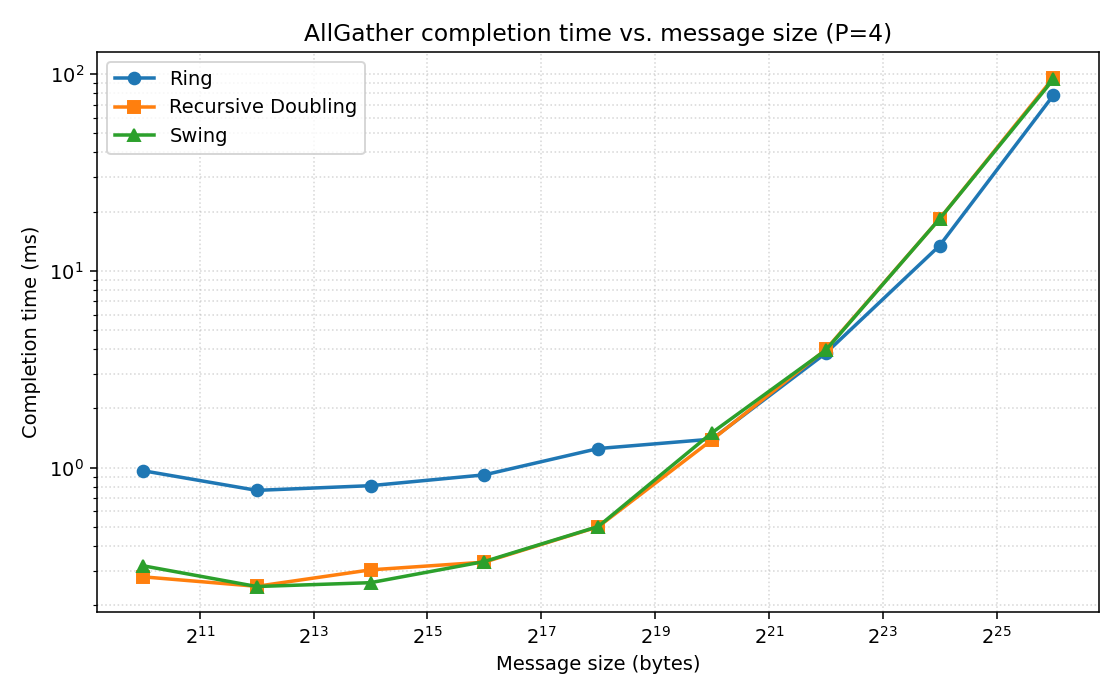
\includegraphics[width=0.85\linewidth]{plots/allgather_vs_size.png}
\end{center}

\begin{itemize}
  \item Below $\sim$1 MiB the \textbf{ring} is $\sim$3$\times$ slower than recursive doubling or
        swing. With $P = 4$ the ring uses $P - 1 = 3$ sequential send/recv
        rounds versus $\log_2 P = 2$ for the others, and at small sizes time is
        dominated by per-round latency --- so the ring pays the extra round.
  \item From $\sim$4 MiB up all three lines converge; every algorithm moves the
        same total bytes per rank, and once the per-message latency is
        amortised the wire time dominates.
  \item Above 16 MiB the \textbf{ring actually wins slightly} ($\sim$78 ms vs.\ $\sim$94 ms
        at 64 MiB). Recursive doubling and swing contiguously exchange
        ever-larger blocks; the ring keeps each round's message at the
        original chunk size, which gives the NIC/TCP stack smaller, more
        pipelineable messages. This pipelining advantage is the classical
        argument for the ring at bandwidth-bound sizes.
\end{itemize}

\subsection{AllGather vs.\ process count (message = 4 MiB)}

\begin{center}
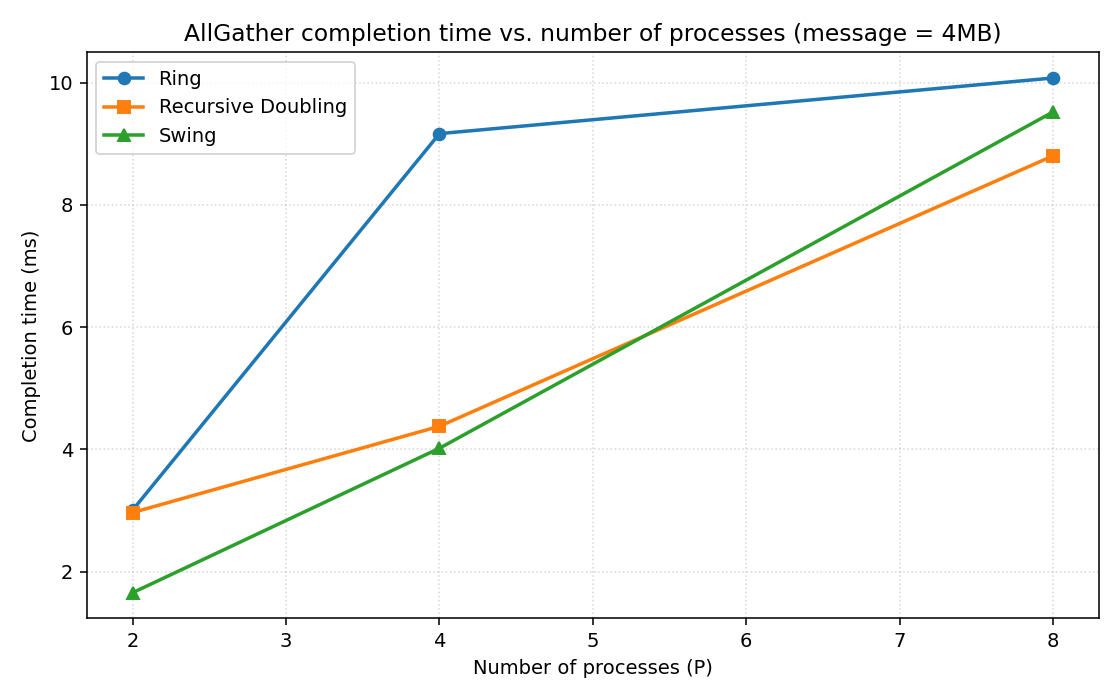
\includegraphics[width=0.85\linewidth]{plots/allgather_vs_ranks.png}
\end{center}

\begin{itemize}
  \item At $P = 2$ all three algorithms do exactly one exchange; times match
        ($\sim$1.7--3.0 ms, variation is measurement noise).
  \item At $P = 4$ the ring takes 9.2 ms, $\sim$2$\times$ recursive doubling / swing,
        matching the $\log P$ vs.\ $P - 1$ round counts.
  \item At $P = 8$ all three converge around 9--10 ms: data per rank has grown
        to $(P - 1)\cdot C$ regardless of algorithm and loopback bandwidth saturates.
\end{itemize}

\subsection{Broadcast vs.\ message size (P = 4)}

\begin{center}
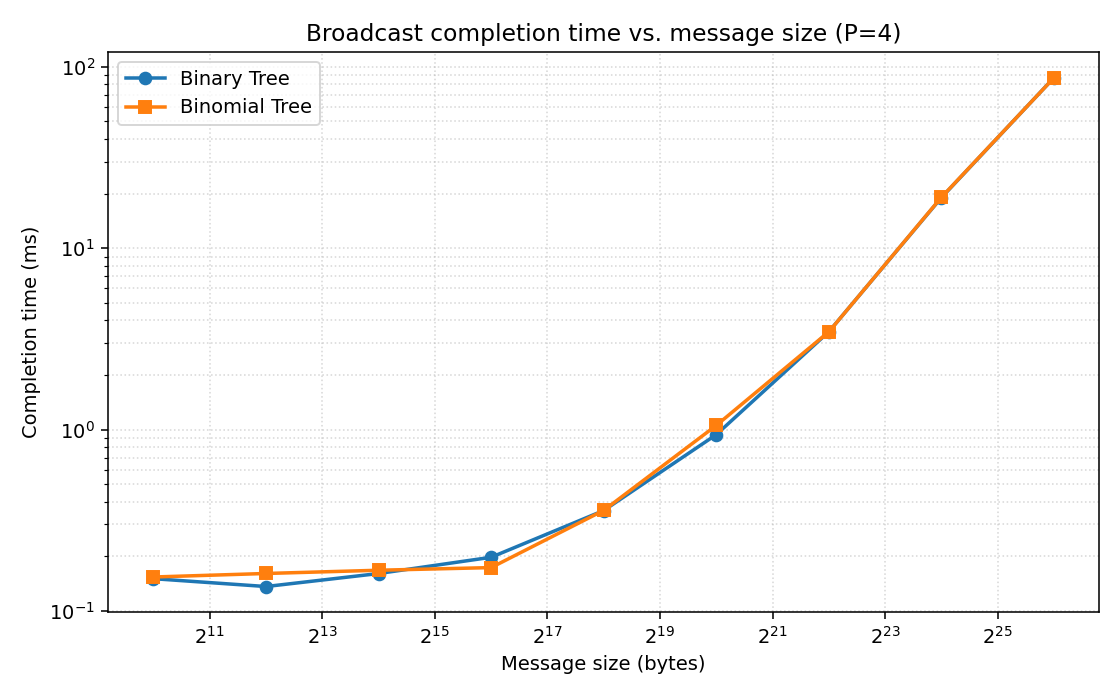
\includegraphics[width=0.85\linewidth]{plots/broadcast_vs_size.png}
\end{center}

\begin{itemize}
  \item Binary tree and binomial tree are within measurement noise across
        the whole range. At $P = 4$ both have depth 2; the binary tree's root
        has fan-out 2 (sends sequentially to children 1 and 2); the
        binomial tree's root also sends twice (at round 0 to rank 1, at
        round 1 to rank 2). Identical amount of serialised work at the root
        means identical completion time.
\end{itemize}

\subsection{Broadcast vs.\ process count (message = 4 MiB)}

\begin{center}
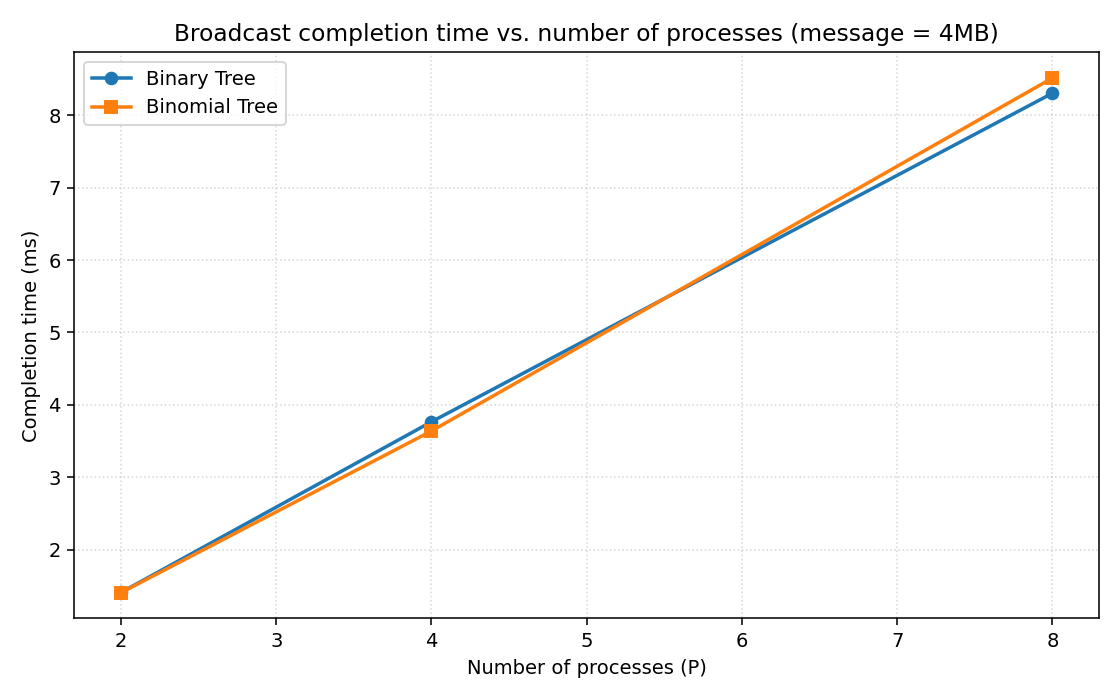
\includegraphics[width=0.85\linewidth]{plots/broadcast_vs_ranks.png}
\end{center}

\begin{itemize}
  \item Both trees scale like $\lceil \log_2 P \rceil \cdot (\text{message} / \text{bandwidth})$ plus a constant
        latency per hop. $P = 2 \to 1$ hop, $P = 4 \to 2$ hops, $P = 8 \to 3$ hops;
        times grow roughly linearly with the hop count (1.4 $\to$ 3.7 $\to$ 8.4 ms).
  \item Again binary and binomial trees overlap --- the two trees have the
        same depth on $P = 2^n$, and on our single-host fabric the difference
        in internal fan-out doesn't translate into different wall-clock
        because each rank's send is serialised against the others.
\end{itemize}

\section{Summary}

\begin{itemize}
  \item \textbf{Small messages (latency-dominated):} log-depth algorithms
        (recursive doubling, swing, both trees) beat the ring on AllGather.
  \item \textbf{Large messages (bandwidth-dominated):} the ring catches up and
        can even win on AllGather thanks to smaller, pipelineable messages;
        tree depth stops mattering for broadcast because each hop carries
        the full payload.
  \item The two broadcast trees we compared are essentially equivalent in
        steady state on a flat fabric; their differences would show up on
        hierarchical or heterogeneous networks, which loopback is not.
\end{itemize}

\section{File manifest}

\begin{Verbatim}[fontsize=\small]
Networks Assignment 5/
|-- collectives.py         # the five algorithms
|-- test_correctness.py    # correctness tests (all pass)
|-- run_experiments.py     # experiment driver
|-- plot_results.py        # plotting
|-- results.json           # raw timing data
|-- experiment_log.txt     # stdout of run_experiments
|-- plots/
|   |-- allgather_vs_size.png
|   |-- allgather_vs_ranks.png
|   |-- broadcast_vs_size.png
|   `-- broadcast_vs_ranks.png
`-- report.md              # markdown source of this report
\end{Verbatim}

Source code and full history are available at
\href{\repourl}{\repourl}.

\section{How to reproduce}

\begin{Verbatim}[fontsize=\small]
# clone the repository
git clone https://github.com/arav-p/networks-assignment-5.git
cd networks-assignment-5

# correctness
python3 test_correctness.py

# experiments (defaults match those reported above)
python3 run_experiments.py \
    --max-bytes $((64*1024*1024)) \
    --max-ranks 8 \
    --fixed-size $((4*1024*1024)) \
    --fixed-ranks 4

# plots
python3 plot_results.py
\end{Verbatim}

\end{document}
